% Created by tikzDevice version 0.8.1 on 2015-03-26 23:37:37
% !TEX encoding = UTF-8 Unicode
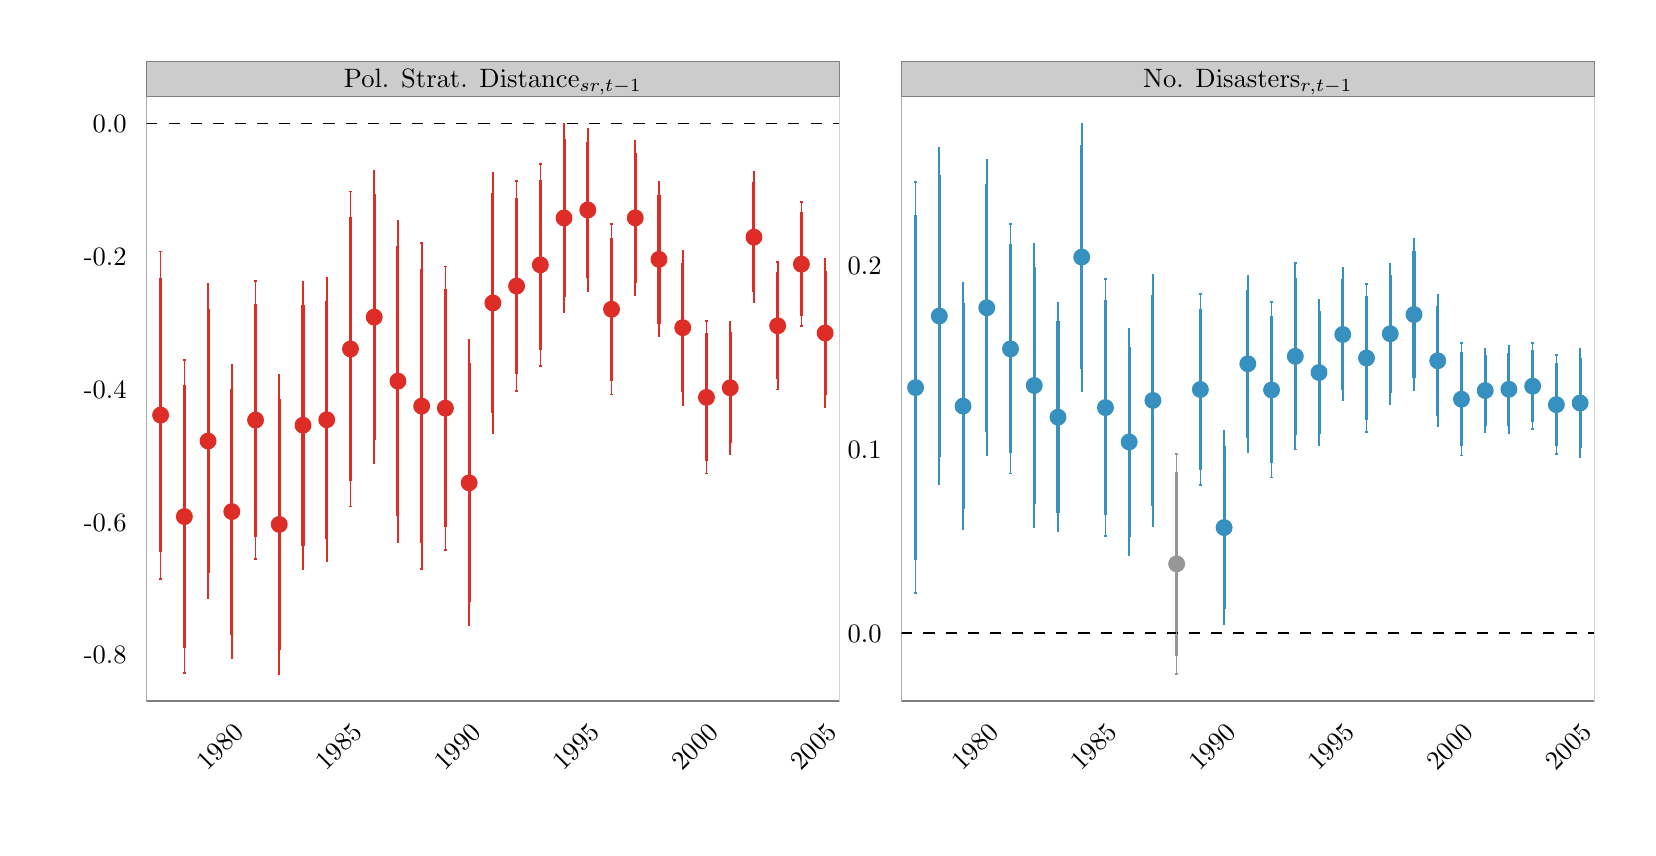
\begin{tikzpicture}[x=1pt,y=1pt]
\definecolor{fillColor}{RGB}{255,255,255}
\path[use as bounding box,fill=fillColor,fill opacity=0.00] (0,0) rectangle (578.16,289.08);
\begin{scope}
\path[clip] (  0.00,  0.00) rectangle (578.16,289.08);
\definecolor{drawColor}{RGB}{255,255,255}
\definecolor{fillColor}{RGB}{255,255,255}

\path[draw=drawColor,line width= 0.6pt,line join=round,line cap=round,fill=fillColor] (  0.00,  0.00) rectangle (578.16,289.08);
\end{scope}
\begin{scope}
\path[clip] ( 42.89, 45.67) rectangle (293.31,264.40);
\definecolor{fillColor}{RGB}{255,255,255}

\path[fill=fillColor] ( 42.89, 45.67) rectangle (293.31,264.40);
\definecolor{drawColor}{RGB}{222,45,38}

\path[draw=drawColor,draw opacity=0.30,line width= 0.3pt,line join=round] ( 48.03, 89.96) -- ( 48.03,208.22);

\path[draw=drawColor,draw opacity=0.30,line width= 0.3pt,line join=round] ( 56.61, 55.94) -- ( 56.61,168.89);

\path[draw=drawColor,draw opacity=0.30,line width= 0.3pt,line join=round] ( 65.18, 82.91) -- ( 65.18,196.49);

\path[draw=drawColor,draw opacity=0.30,line width= 0.3pt,line join=round] ( 73.76, 61.21) -- ( 73.76,167.21);

\path[draw=drawColor,draw opacity=0.30,line width= 0.3pt,line join=round] ( 82.34, 97.13) -- ( 82.34,197.44);

\path[draw=drawColor,draw opacity=0.30,line width= 0.3pt,line join=round] ( 90.91, 55.61) -- ( 90.91,163.55);

\path[draw=drawColor,draw opacity=0.30,line width= 0.3pt,line join=round] ( 99.49, 93.57) -- ( 99.49,197.27);

\path[draw=drawColor,draw opacity=0.30,line width= 0.3pt,line join=round] (108.06, 96.12) -- (108.06,198.68);

\path[draw=drawColor,draw opacity=0.30,line width= 0.3pt,line join=round] (116.64,116.01) -- (116.64,229.92);

\path[draw=drawColor,draw opacity=0.30,line width= 0.3pt,line join=round] (125.22,131.64) -- (125.22,237.35);

\path[draw=drawColor,draw opacity=0.30,line width= 0.3pt,line join=round] (133.79,103.34) -- (133.79,219.35);

\path[draw=drawColor,draw opacity=0.30,line width= 0.3pt,line join=round] (142.37, 93.47) -- (142.37,211.17);

\path[draw=drawColor,draw opacity=0.30,line width= 0.3pt,line join=round] (150.94,100.38) -- (150.94,202.76);

\path[draw=drawColor,draw opacity=0.30,line width= 0.3pt,line join=round] (159.52, 73.11) -- (159.52,176.11);

\path[draw=drawColor,draw opacity=0.30,line width= 0.3pt,line join=round] (168.10,142.41) -- (168.10,236.79);

\path[draw=drawColor,draw opacity=0.30,line width= 0.3pt,line join=round] (176.67,157.86) -- (176.67,233.56);

\path[draw=drawColor,draw opacity=0.30,line width= 0.3pt,line join=round] (185.25,166.82) -- (185.25,239.93);

\path[draw=drawColor,draw opacity=0.30,line width= 0.3pt,line join=round] (193.82,186.38) -- (193.82,254.25);

\path[draw=drawColor,draw opacity=0.30,line width= 0.3pt,line join=round] (202.40,193.76) -- (202.40,252.64);

\path[draw=drawColor,draw opacity=0.30,line width= 0.3pt,line join=round] (210.98,156.50) -- (210.98,218.15);

\path[draw=drawColor,draw opacity=0.30,line width= 0.3pt,line join=round] (219.55,192.41) -- (219.55,248.29);

\path[draw=drawColor,draw opacity=0.30,line width= 0.3pt,line join=round] (228.13,177.46) -- (228.13,233.26);

\path[draw=drawColor,draw opacity=0.30,line width= 0.3pt,line join=round] (236.70,152.79) -- (236.70,208.56);

\path[draw=drawColor,draw opacity=0.30,line width= 0.3pt,line join=round] (245.28,127.96) -- (245.28,183.01);

\path[draw=drawColor,draw opacity=0.30,line width= 0.3pt,line join=round] (253.86,135.12) -- (253.86,182.76);

\path[draw=drawColor,draw opacity=0.30,line width= 0.3pt,line join=round] (262.43,189.73) -- (262.43,237.05);

\path[draw=drawColor,draw opacity=0.30,line width= 0.3pt,line join=round] (271.01,158.31) -- (271.01,204.38);

\path[draw=drawColor,draw opacity=0.30,line width= 0.3pt,line join=round] (279.58,181.27) -- (279.58,225.98);

\path[draw=drawColor,draw opacity=0.30,line width= 0.3pt,line join=round] (288.16,151.94) -- (288.16,205.54);
\definecolor{drawColor}{RGB}{222,45,38}

\path[draw=drawColor,line width= 1.1pt,line join=round] ( 48.03, 99.47) -- ( 48.03,198.71);

\path[draw=drawColor,line width= 1.1pt,line join=round] ( 56.61, 65.02) -- ( 56.61,159.81);

\path[draw=drawColor,line width= 1.1pt,line join=round] ( 65.18, 92.04) -- ( 65.18,187.36);

\path[draw=drawColor,line width= 1.1pt,line join=round] ( 73.76, 69.73) -- ( 73.76,158.69);

\path[draw=drawColor,line width= 1.1pt,line join=round] ( 82.34,105.19) -- ( 82.34,189.38);

\path[draw=drawColor,line width= 1.1pt,line join=round] ( 90.91, 64.29) -- ( 90.91,154.88);

\path[draw=drawColor,line width= 1.1pt,line join=round] ( 99.49,101.91) -- ( 99.49,188.94);

\path[draw=drawColor,line width= 1.1pt,line join=round] (108.06,104.37) -- (108.06,190.44);

\path[draw=drawColor,line width= 1.1pt,line join=round] (116.64,125.16) -- (116.64,220.77);

\path[draw=drawColor,line width= 1.1pt,line join=round] (125.22,140.14) -- (125.22,228.85);

\path[draw=drawColor,line width= 1.1pt,line join=round] (133.79,112.67) -- (133.79,210.03);

\path[draw=drawColor,line width= 1.1pt,line join=round] (142.37,102.93) -- (142.37,201.71);

\path[draw=drawColor,line width= 1.1pt,line join=round] (150.94,108.61) -- (150.94,194.53);

\path[draw=drawColor,line width= 1.1pt,line join=round] (159.52, 81.39) -- (159.52,167.83);

\path[draw=drawColor,line width= 1.1pt,line join=round] (168.10,149.99) -- (168.10,229.21);

\path[draw=drawColor,line width= 1.1pt,line join=round] (176.67,163.95) -- (176.67,227.47);

\path[draw=drawColor,line width= 1.1pt,line join=round] (185.25,172.69) -- (185.25,234.05);

\path[draw=drawColor,line width= 1.1pt,line join=round] (193.82,191.84) -- (193.82,248.79);

\path[draw=drawColor,line width= 1.1pt,line join=round] (202.40,198.50) -- (202.40,247.91);

\path[draw=drawColor,line width= 1.1pt,line join=round] (210.98,161.46) -- (210.98,213.19);

\path[draw=drawColor,line width= 1.1pt,line join=round] (219.55,196.90) -- (219.55,243.80);

\path[draw=drawColor,line width= 1.1pt,line join=round] (228.13,181.94) -- (228.13,228.78);

\path[draw=drawColor,line width= 1.1pt,line join=round] (236.70,157.27) -- (236.70,204.08);

\path[draw=drawColor,line width= 1.1pt,line join=round] (245.28,132.39) -- (245.28,178.59);

\path[draw=drawColor,line width= 1.1pt,line join=round] (253.86,138.95) -- (253.86,178.93);

\path[draw=drawColor,line width= 1.1pt,line join=round] (262.43,193.54) -- (262.43,233.25);

\path[draw=drawColor,line width= 1.1pt,line join=round] (271.01,162.01) -- (271.01,200.68);

\path[draw=drawColor,line width= 1.1pt,line join=round] (279.58,184.86) -- (279.58,222.39);

\path[draw=drawColor,line width= 1.1pt,line join=round] (288.16,156.25) -- (288.16,201.23);
\definecolor{drawColor}{RGB}{0,0,0}

\path[draw=drawColor,line width= 0.6pt,dash pattern=on 4pt off 4pt ,line join=round] ( 42.89,254.46) -- (293.31,254.46);
\definecolor{drawColor}{RGB}{222,45,38}
\definecolor{fillColor}{RGB}{222,45,38}

\path[draw=drawColor,line width= 0.4pt,line join=round,line cap=round,fill=fillColor] ( 48.03,149.09) circle (  2.85);

\path[draw=drawColor,line width= 0.4pt,line join=round,line cap=round,fill=fillColor] ( 56.61,112.42) circle (  2.85);

\path[draw=drawColor,line width= 0.4pt,line join=round,line cap=round,fill=fillColor] ( 65.18,139.70) circle (  2.85);

\path[draw=drawColor,line width= 0.4pt,line join=round,line cap=round,fill=fillColor] ( 73.76,114.21) circle (  2.85);

\path[draw=drawColor,line width= 0.4pt,line join=round,line cap=round,fill=fillColor] ( 82.34,147.29) circle (  2.85);

\path[draw=drawColor,line width= 0.4pt,line join=round,line cap=round,fill=fillColor] ( 90.91,109.58) circle (  2.85);

\path[draw=drawColor,line width= 0.4pt,line join=round,line cap=round,fill=fillColor] ( 99.49,145.42) circle (  2.85);

\path[draw=drawColor,line width= 0.4pt,line join=round,line cap=round,fill=fillColor] (108.06,147.40) circle (  2.85);

\path[draw=drawColor,line width= 0.4pt,line join=round,line cap=round,fill=fillColor] (116.64,172.97) circle (  2.85);

\path[draw=drawColor,line width= 0.4pt,line join=round,line cap=round,fill=fillColor] (125.22,184.49) circle (  2.85);

\path[draw=drawColor,line width= 0.4pt,line join=round,line cap=round,fill=fillColor] (133.79,161.35) circle (  2.85);

\path[draw=drawColor,line width= 0.4pt,line join=round,line cap=round,fill=fillColor] (142.37,152.32) circle (  2.85);

\path[draw=drawColor,line width= 0.4pt,line join=round,line cap=round,fill=fillColor] (150.94,151.57) circle (  2.85);

\path[draw=drawColor,line width= 0.4pt,line join=round,line cap=round,fill=fillColor] (159.52,124.61) circle (  2.85);

\path[draw=drawColor,line width= 0.4pt,line join=round,line cap=round,fill=fillColor] (168.10,189.60) circle (  2.85);

\path[draw=drawColor,line width= 0.4pt,line join=round,line cap=round,fill=fillColor] (176.67,195.71) circle (  2.85);

\path[draw=drawColor,line width= 0.4pt,line join=round,line cap=round,fill=fillColor] (185.25,203.37) circle (  2.85);

\path[draw=drawColor,line width= 0.4pt,line join=round,line cap=round,fill=fillColor] (193.82,220.32) circle (  2.85);

\path[draw=drawColor,line width= 0.4pt,line join=round,line cap=round,fill=fillColor] (202.40,223.20) circle (  2.85);

\path[draw=drawColor,line width= 0.4pt,line join=round,line cap=round,fill=fillColor] (210.98,187.33) circle (  2.85);

\path[draw=drawColor,line width= 0.4pt,line join=round,line cap=round,fill=fillColor] (219.55,220.35) circle (  2.85);

\path[draw=drawColor,line width= 0.4pt,line join=round,line cap=round,fill=fillColor] (228.13,205.36) circle (  2.85);

\path[draw=drawColor,line width= 0.4pt,line join=round,line cap=round,fill=fillColor] (236.70,180.67) circle (  2.85);

\path[draw=drawColor,line width= 0.4pt,line join=round,line cap=round,fill=fillColor] (245.28,155.49) circle (  2.85);

\path[draw=drawColor,line width= 0.4pt,line join=round,line cap=round,fill=fillColor] (253.86,158.94) circle (  2.85);

\path[draw=drawColor,line width= 0.4pt,line join=round,line cap=round,fill=fillColor] (262.43,213.39) circle (  2.85);

\path[draw=drawColor,line width= 0.4pt,line join=round,line cap=round,fill=fillColor] (271.01,181.35) circle (  2.85);

\path[draw=drawColor,line width= 0.4pt,line join=round,line cap=round,fill=fillColor] (279.58,203.62) circle (  2.85);

\path[draw=drawColor,line width= 0.4pt,line join=round,line cap=round,fill=fillColor] (288.16,178.74) circle (  2.85);

\path[draw=drawColor,line width= 0.6pt,line join=round] ( 47.60,208.22) --
	( 48.46,208.22);

\path[draw=drawColor,line width= 0.6pt,line join=round] ( 48.03,208.22) --
	( 48.03, 89.96);

\path[draw=drawColor,line width= 0.6pt,line join=round] ( 47.60, 89.96) --
	( 48.46, 89.96);

\path[draw=drawColor,line width= 0.6pt,line join=round] ( 56.18,168.89) --
	( 57.04,168.89);

\path[draw=drawColor,line width= 0.6pt,line join=round] ( 56.61,168.89) --
	( 56.61, 55.94);

\path[draw=drawColor,line width= 0.6pt,line join=round] ( 56.18, 55.94) --
	( 57.04, 55.94);

\path[draw=drawColor,line width= 0.6pt,line join=round] ( 64.75,196.49) --
	( 65.61,196.49);

\path[draw=drawColor,line width= 0.6pt,line join=round] ( 65.18,196.49) --
	( 65.18, 82.91);

\path[draw=drawColor,line width= 0.6pt,line join=round] ( 64.75, 82.91) --
	( 65.61, 82.91);

\path[draw=drawColor,line width= 0.6pt,line join=round] ( 73.33,167.21) --
	( 74.19,167.21);

\path[draw=drawColor,line width= 0.6pt,line join=round] ( 73.76,167.21) --
	( 73.76, 61.21);

\path[draw=drawColor,line width= 0.6pt,line join=round] ( 73.33, 61.21) --
	( 74.19, 61.21);

\path[draw=drawColor,line width= 0.6pt,line join=round] ( 81.91,197.44) --
	( 82.76,197.44);

\path[draw=drawColor,line width= 0.6pt,line join=round] ( 82.34,197.44) --
	( 82.34, 97.13);

\path[draw=drawColor,line width= 0.6pt,line join=round] ( 81.91, 97.13) --
	( 82.76, 97.13);

\path[draw=drawColor,line width= 0.6pt,line join=round] ( 90.48,163.55) --
	( 91.34,163.55);

\path[draw=drawColor,line width= 0.6pt,line join=round] ( 90.91,163.55) --
	( 90.91, 55.61);

\path[draw=drawColor,line width= 0.6pt,line join=round] ( 90.48, 55.61) --
	( 91.34, 55.61);

\path[draw=drawColor,line width= 0.6pt,line join=round] ( 99.06,197.27) --
	( 99.92,197.27);

\path[draw=drawColor,line width= 0.6pt,line join=round] ( 99.49,197.27) --
	( 99.49, 93.57);

\path[draw=drawColor,line width= 0.6pt,line join=round] ( 99.06, 93.57) --
	( 99.92, 93.57);

\path[draw=drawColor,line width= 0.6pt,line join=round] (107.63,198.68) --
	(108.49,198.68);

\path[draw=drawColor,line width= 0.6pt,line join=round] (108.06,198.68) --
	(108.06, 96.12);

\path[draw=drawColor,line width= 0.6pt,line join=round] (107.63, 96.12) --
	(108.49, 96.12);

\path[draw=drawColor,line width= 0.6pt,line join=round] (116.21,229.92) --
	(117.07,229.92);

\path[draw=drawColor,line width= 0.6pt,line join=round] (116.64,229.92) --
	(116.64,116.01);

\path[draw=drawColor,line width= 0.6pt,line join=round] (116.21,116.01) --
	(117.07,116.01);

\path[draw=drawColor,line width= 0.6pt,line join=round] (124.79,237.35) --
	(125.64,237.35);

\path[draw=drawColor,line width= 0.6pt,line join=round] (125.22,237.35) --
	(125.22,131.64);

\path[draw=drawColor,line width= 0.6pt,line join=round] (124.79,131.64) --
	(125.64,131.64);

\path[draw=drawColor,line width= 0.6pt,line join=round] (133.36,219.35) --
	(134.22,219.35);

\path[draw=drawColor,line width= 0.6pt,line join=round] (133.79,219.35) --
	(133.79,103.34);

\path[draw=drawColor,line width= 0.6pt,line join=round] (133.36,103.34) --
	(134.22,103.34);

\path[draw=drawColor,line width= 0.6pt,line join=round] (141.94,211.17) --
	(142.80,211.17);

\path[draw=drawColor,line width= 0.6pt,line join=round] (142.37,211.17) --
	(142.37, 93.47);

\path[draw=drawColor,line width= 0.6pt,line join=round] (141.94, 93.47) --
	(142.80, 93.47);

\path[draw=drawColor,line width= 0.6pt,line join=round] (150.52,202.76) --
	(151.37,202.76);

\path[draw=drawColor,line width= 0.6pt,line join=round] (150.94,202.76) --
	(150.94,100.38);

\path[draw=drawColor,line width= 0.6pt,line join=round] (150.52,100.38) --
	(151.37,100.38);

\path[draw=drawColor,line width= 0.6pt,line join=round] (159.09,176.11) --
	(159.95,176.11);

\path[draw=drawColor,line width= 0.6pt,line join=round] (159.52,176.11) --
	(159.52, 73.11);

\path[draw=drawColor,line width= 0.6pt,line join=round] (159.09, 73.11) --
	(159.95, 73.11);

\path[draw=drawColor,line width= 0.6pt,line join=round] (167.67,236.79) --
	(168.52,236.79);

\path[draw=drawColor,line width= 0.6pt,line join=round] (168.10,236.79) --
	(168.10,142.41);

\path[draw=drawColor,line width= 0.6pt,line join=round] (167.67,142.41) --
	(168.52,142.41);

\path[draw=drawColor,line width= 0.6pt,line join=round] (176.24,233.56) --
	(177.10,233.56);

\path[draw=drawColor,line width= 0.6pt,line join=round] (176.67,233.56) --
	(176.67,157.86);

\path[draw=drawColor,line width= 0.6pt,line join=round] (176.24,157.86) --
	(177.10,157.86);

\path[draw=drawColor,line width= 0.6pt,line join=round] (184.82,239.93) --
	(185.68,239.93);

\path[draw=drawColor,line width= 0.6pt,line join=round] (185.25,239.93) --
	(185.25,166.82);

\path[draw=drawColor,line width= 0.6pt,line join=round] (184.82,166.82) --
	(185.68,166.82);

\path[draw=drawColor,line width= 0.6pt,line join=round] (193.40,254.25) --
	(194.25,254.25);

\path[draw=drawColor,line width= 0.6pt,line join=round] (193.82,254.25) --
	(193.82,186.38);

\path[draw=drawColor,line width= 0.6pt,line join=round] (193.40,186.38) --
	(194.25,186.38);

\path[draw=drawColor,line width= 0.6pt,line join=round] (201.97,252.64) --
	(202.83,252.64);

\path[draw=drawColor,line width= 0.6pt,line join=round] (202.40,252.64) --
	(202.40,193.76);

\path[draw=drawColor,line width= 0.6pt,line join=round] (201.97,193.76) --
	(202.83,193.76);

\path[draw=drawColor,line width= 0.6pt,line join=round] (210.55,218.15) --
	(211.41,218.15);

\path[draw=drawColor,line width= 0.6pt,line join=round] (210.98,218.15) --
	(210.98,156.50);

\path[draw=drawColor,line width= 0.6pt,line join=round] (210.55,156.50) --
	(211.41,156.50);

\path[draw=drawColor,line width= 0.6pt,line join=round] (219.12,248.29) --
	(219.98,248.29);

\path[draw=drawColor,line width= 0.6pt,line join=round] (219.55,248.29) --
	(219.55,192.41);

\path[draw=drawColor,line width= 0.6pt,line join=round] (219.12,192.41) --
	(219.98,192.41);

\path[draw=drawColor,line width= 0.6pt,line join=round] (227.70,233.26) --
	(228.56,233.26);

\path[draw=drawColor,line width= 0.6pt,line join=round] (228.13,233.26) --
	(228.13,177.46);

\path[draw=drawColor,line width= 0.6pt,line join=round] (227.70,177.46) --
	(228.56,177.46);

\path[draw=drawColor,line width= 0.6pt,line join=round] (236.28,208.56) --
	(237.13,208.56);

\path[draw=drawColor,line width= 0.6pt,line join=round] (236.70,208.56) --
	(236.70,152.79);

\path[draw=drawColor,line width= 0.6pt,line join=round] (236.28,152.79) --
	(237.13,152.79);

\path[draw=drawColor,line width= 0.6pt,line join=round] (244.85,183.01) --
	(245.71,183.01);

\path[draw=drawColor,line width= 0.6pt,line join=round] (245.28,183.01) --
	(245.28,127.96);

\path[draw=drawColor,line width= 0.6pt,line join=round] (244.85,127.96) --
	(245.71,127.96);

\path[draw=drawColor,line width= 0.6pt,line join=round] (253.43,182.76) --
	(254.29,182.76);

\path[draw=drawColor,line width= 0.6pt,line join=round] (253.86,182.76) --
	(253.86,135.12);

\path[draw=drawColor,line width= 0.6pt,line join=round] (253.43,135.12) --
	(254.29,135.12);

\path[draw=drawColor,line width= 0.6pt,line join=round] (262.00,237.05) --
	(262.86,237.05);

\path[draw=drawColor,line width= 0.6pt,line join=round] (262.43,237.05) --
	(262.43,189.73);

\path[draw=drawColor,line width= 0.6pt,line join=round] (262.00,189.73) --
	(262.86,189.73);

\path[draw=drawColor,line width= 0.6pt,line join=round] (270.58,204.38) --
	(271.44,204.38);

\path[draw=drawColor,line width= 0.6pt,line join=round] (271.01,204.38) --
	(271.01,158.31);

\path[draw=drawColor,line width= 0.6pt,line join=round] (270.58,158.31) --
	(271.44,158.31);

\path[draw=drawColor,line width= 0.6pt,line join=round] (279.16,225.98) --
	(280.01,225.98);

\path[draw=drawColor,line width= 0.6pt,line join=round] (279.58,225.98) --
	(279.58,181.27);

\path[draw=drawColor,line width= 0.6pt,line join=round] (279.16,181.27) --
	(280.01,181.27);

\path[draw=drawColor,line width= 0.6pt,line join=round] (287.73,205.54) --
	(288.59,205.54);

\path[draw=drawColor,line width= 0.6pt,line join=round] (288.16,205.54) --
	(288.16,151.94);

\path[draw=drawColor,line width= 0.6pt,line join=round] (287.73,151.94) --
	(288.59,151.94);
\definecolor{drawColor}{gray}{0.50}

\path[draw=drawColor,line width= 0.6pt,line join=round,line cap=round] ( 42.89, 45.67) rectangle (293.31,264.40);
\end{scope}
\begin{scope}
\path[clip] (315.69, 45.67) rectangle (566.12,264.40);
\definecolor{fillColor}{RGB}{255,255,255}

\path[fill=fillColor] (315.69, 45.67) rectangle (566.12,264.40);
\definecolor{drawColor}{RGB}{54,144,192}

\path[draw=drawColor,draw opacity=0.30,line width= 0.3pt,line join=round] (320.84, 84.78) -- (320.84,233.26);

\path[draw=drawColor,draw opacity=0.30,line width= 0.3pt,line join=round] (329.42,124.20) -- (329.42,245.58);

\path[draw=drawColor,draw opacity=0.30,line width= 0.3pt,line join=round] (337.99,107.85) -- (337.99,196.79);

\path[draw=drawColor,draw opacity=0.30,line width= 0.3pt,line join=round] (346.57,134.53) -- (346.57,241.19);

\path[draw=drawColor,draw opacity=0.30,line width= 0.3pt,line join=round] (355.14,128.00) -- (355.14,218.02);

\path[draw=drawColor,draw opacity=0.30,line width= 0.3pt,line join=round] (363.72,108.61) -- (363.72,210.96);

\path[draw=drawColor,draw opacity=0.30,line width= 0.3pt,line join=round] (372.30,107.10) -- (372.30,189.58);

\path[draw=drawColor,draw opacity=0.30,line width= 0.3pt,line join=round] (380.87,157.89) -- (380.87,254.46);

\path[draw=drawColor,draw opacity=0.30,line width= 0.3pt,line join=round] (389.45,105.38) -- (389.45,198.20);

\path[draw=drawColor,draw opacity=0.30,line width= 0.3pt,line join=round] (398.02, 98.44) -- (398.02,180.32);

\path[draw=drawColor,draw opacity=0.30,line width= 0.3pt,line join=round] (406.60,108.83) -- (406.60,199.93);
\definecolor{drawColor}{RGB}{150,150,150}

\path[draw=drawColor,draw opacity=0.30,line width= 0.3pt,line join=round] (415.18, 55.61) -- (415.18,135.03);
\definecolor{drawColor}{RGB}{54,144,192}

\path[draw=drawColor,draw opacity=0.30,line width= 0.3pt,line join=round] (423.75,123.82) -- (423.75,192.84);

\path[draw=drawColor,draw opacity=0.30,line width= 0.3pt,line join=round] (432.33, 73.48) -- (432.33,143.39);

\path[draw=drawColor,draw opacity=0.30,line width= 0.3pt,line join=round] (440.90,135.71) -- (440.90,199.57);

\path[draw=drawColor,draw opacity=0.30,line width= 0.3pt,line join=round] (449.48,126.51) -- (449.48,189.85);

\path[draw=drawColor,draw opacity=0.30,line width= 0.3pt,line join=round] (458.06,136.62) -- (458.06,204.01);

\path[draw=drawColor,draw opacity=0.30,line width= 0.3pt,line join=round] (466.63,138.09) -- (466.63,190.85);

\path[draw=drawColor,draw opacity=0.30,line width= 0.3pt,line join=round] (475.21,154.32) -- (475.21,202.12);

\path[draw=drawColor,draw opacity=0.30,line width= 0.3pt,line join=round] (483.78,143.07) -- (483.78,196.36);

\path[draw=drawColor,draw opacity=0.30,line width= 0.3pt,line join=round] (492.36,153.05) -- (492.36,203.91);

\path[draw=drawColor,draw opacity=0.30,line width= 0.3pt,line join=round] (500.94,158.05) -- (500.94,212.80);

\path[draw=drawColor,draw opacity=0.30,line width= 0.3pt,line join=round] (509.51,145.03) -- (509.51,192.41);

\path[draw=drawColor,draw opacity=0.30,line width= 0.3pt,line join=round] (518.09,134.49) -- (518.09,175.12);

\path[draw=drawColor,draw opacity=0.30,line width= 0.3pt,line join=round] (526.67,142.74) -- (526.67,173.16);

\path[draw=drawColor,draw opacity=0.30,line width= 0.3pt,line join=round] (535.24,142.56) -- (535.24,174.24);

\path[draw=drawColor,draw opacity=0.30,line width= 0.3pt,line join=round] (543.82,143.99) -- (543.82,175.07);

\path[draw=drawColor,draw opacity=0.30,line width= 0.3pt,line join=round] (552.39,134.95) -- (552.39,170.75);

\path[draw=drawColor,draw opacity=0.30,line width= 0.3pt,line join=round] (560.97,134.02) -- (560.97,172.88);
\definecolor{drawColor}{RGB}{54,144,192}

\path[draw=drawColor,line width= 1.1pt,line join=round] (320.84, 96.72) -- (320.84,221.32);

\path[draw=drawColor,line width= 1.1pt,line join=round] (329.42,133.96) -- (329.42,235.83);

\path[draw=drawColor,line width= 1.1pt,line join=round] (337.99,115.00) -- (337.99,189.64);

\path[draw=drawColor,line width= 1.1pt,line join=round] (346.57,143.11) -- (346.57,232.62);

\path[draw=drawColor,line width= 1.1pt,line join=round] (355.14,135.23) -- (355.14,210.79);

\path[draw=drawColor,line width= 1.1pt,line join=round] (363.72,116.84) -- (363.72,202.73);

\path[draw=drawColor,line width= 1.1pt,line join=round] (372.30,113.73) -- (372.30,182.95);

\path[draw=drawColor,line width= 1.1pt,line join=round] (380.87,165.65) -- (380.87,246.70);

\path[draw=drawColor,line width= 1.1pt,line join=round] (389.45,112.84) -- (389.45,190.74);

\path[draw=drawColor,line width= 1.1pt,line join=round] (398.02,105.02) -- (398.02,173.74);

\path[draw=drawColor,line width= 1.1pt,line join=round] (406.60,116.15) -- (406.60,192.61);
\definecolor{drawColor}{gray}{0.59}

\path[draw=drawColor,line width= 1.1pt,line join=round] (415.18, 62.00) -- (415.18,128.64);
\definecolor{drawColor}{RGB}{54,144,192}

\path[draw=drawColor,line width= 1.1pt,line join=round] (423.75,129.37) -- (423.75,187.29);

\path[draw=drawColor,line width= 1.1pt,line join=round] (432.33, 79.10) -- (432.33,137.77);

\path[draw=drawColor,line width= 1.1pt,line join=round] (440.90,140.84) -- (440.90,194.44);

\path[draw=drawColor,line width= 1.1pt,line join=round] (449.48,131.60) -- (449.48,184.76);

\path[draw=drawColor,line width= 1.1pt,line join=round] (458.06,142.04) -- (458.06,198.59);

\path[draw=drawColor,line width= 1.1pt,line join=round] (466.63,142.33) -- (466.63,186.61);

\path[draw=drawColor,line width= 1.1pt,line join=round] (475.21,158.17) -- (475.21,198.28);

\path[draw=drawColor,line width= 1.1pt,line join=round] (483.78,147.36) -- (483.78,192.07);

\path[draw=drawColor,line width= 1.1pt,line join=round] (492.36,157.14) -- (492.36,199.82);

\path[draw=drawColor,line width= 1.1pt,line join=round] (500.94,162.45) -- (500.94,208.40);

\path[draw=drawColor,line width= 1.1pt,line join=round] (509.51,148.84) -- (509.51,188.60);

\path[draw=drawColor,line width= 1.1pt,line join=round] (518.09,137.76) -- (518.09,171.86);

\path[draw=drawColor,line width= 1.1pt,line join=round] (526.67,145.19) -- (526.67,170.71);

\path[draw=drawColor,line width= 1.1pt,line join=round] (535.24,145.11) -- (535.24,171.69);

\path[draw=drawColor,line width= 1.1pt,line join=round] (543.82,146.49) -- (543.82,172.57);

\path[draw=drawColor,line width= 1.1pt,line join=round] (552.39,137.83) -- (552.39,167.87);

\path[draw=drawColor,line width= 1.1pt,line join=round] (560.97,137.14) -- (560.97,169.75);
\definecolor{drawColor}{RGB}{0,0,0}

\path[draw=drawColor,line width= 0.6pt,dash pattern=on 4pt off 4pt ,line join=round] (315.69, 70.25) -- (566.12, 70.25);
\definecolor{drawColor}{RGB}{54,144,192}
\definecolor{fillColor}{RGB}{54,144,192}

\path[draw=drawColor,line width= 0.4pt,line join=round,line cap=round,fill=fillColor] (320.84,159.02) circle (  2.85);

\path[draw=drawColor,line width= 0.4pt,line join=round,line cap=round,fill=fillColor] (329.42,184.89) circle (  2.85);

\path[draw=drawColor,line width= 0.4pt,line join=round,line cap=round,fill=fillColor] (337.99,152.32) circle (  2.85);

\path[draw=drawColor,line width= 0.4pt,line join=round,line cap=round,fill=fillColor] (346.57,187.86) circle (  2.85);

\path[draw=drawColor,line width= 0.4pt,line join=round,line cap=round,fill=fillColor] (355.14,173.01) circle (  2.85);

\path[draw=drawColor,line width= 0.4pt,line join=round,line cap=round,fill=fillColor] (363.72,159.79) circle (  2.85);

\path[draw=drawColor,line width= 0.4pt,line join=round,line cap=round,fill=fillColor] (372.30,148.34) circle (  2.85);

\path[draw=drawColor,line width= 0.4pt,line join=round,line cap=round,fill=fillColor] (380.87,206.17) circle (  2.85);

\path[draw=drawColor,line width= 0.4pt,line join=round,line cap=round,fill=fillColor] (389.45,151.79) circle (  2.85);

\path[draw=drawColor,line width= 0.4pt,line join=round,line cap=round,fill=fillColor] (398.02,139.38) circle (  2.85);

\path[draw=drawColor,line width= 0.4pt,line join=round,line cap=round,fill=fillColor] (406.60,154.38) circle (  2.85);
\definecolor{drawColor}{gray}{0.59}
\definecolor{fillColor}{gray}{0.59}

\path[draw=drawColor,line width= 0.4pt,line join=round,line cap=round,fill=fillColor] (415.18, 95.32) circle (  2.85);
\definecolor{drawColor}{RGB}{54,144,192}
\definecolor{fillColor}{RGB}{54,144,192}

\path[draw=drawColor,line width= 0.4pt,line join=round,line cap=round,fill=fillColor] (423.75,158.33) circle (  2.85);

\path[draw=drawColor,line width= 0.4pt,line join=round,line cap=round,fill=fillColor] (432.33,108.43) circle (  2.85);

\path[draw=drawColor,line width= 0.4pt,line join=round,line cap=round,fill=fillColor] (440.90,167.64) circle (  2.85);

\path[draw=drawColor,line width= 0.4pt,line join=round,line cap=round,fill=fillColor] (449.48,158.18) circle (  2.85);

\path[draw=drawColor,line width= 0.4pt,line join=round,line cap=round,fill=fillColor] (458.06,170.32) circle (  2.85);

\path[draw=drawColor,line width= 0.4pt,line join=round,line cap=round,fill=fillColor] (466.63,164.47) circle (  2.85);

\path[draw=drawColor,line width= 0.4pt,line join=round,line cap=round,fill=fillColor] (475.21,178.22) circle (  2.85);

\path[draw=drawColor,line width= 0.4pt,line join=round,line cap=round,fill=fillColor] (483.78,169.72) circle (  2.85);

\path[draw=drawColor,line width= 0.4pt,line join=round,line cap=round,fill=fillColor] (492.36,178.48) circle (  2.85);

\path[draw=drawColor,line width= 0.4pt,line join=round,line cap=round,fill=fillColor] (500.94,185.42) circle (  2.85);

\path[draw=drawColor,line width= 0.4pt,line join=round,line cap=round,fill=fillColor] (509.51,168.72) circle (  2.85);

\path[draw=drawColor,line width= 0.4pt,line join=round,line cap=round,fill=fillColor] (518.09,154.81) circle (  2.85);

\path[draw=drawColor,line width= 0.4pt,line join=round,line cap=round,fill=fillColor] (526.67,157.95) circle (  2.85);

\path[draw=drawColor,line width= 0.4pt,line join=round,line cap=round,fill=fillColor] (535.24,158.40) circle (  2.85);

\path[draw=drawColor,line width= 0.4pt,line join=round,line cap=round,fill=fillColor] (543.82,159.53) circle (  2.85);

\path[draw=drawColor,line width= 0.4pt,line join=round,line cap=round,fill=fillColor] (552.39,152.85) circle (  2.85);

\path[draw=drawColor,line width= 0.4pt,line join=round,line cap=round,fill=fillColor] (560.97,153.45) circle (  2.85);

\path[draw=drawColor,line width= 0.6pt,line join=round] (320.41,233.26) --
	(321.27,233.26);

\path[draw=drawColor,line width= 0.6pt,line join=round] (320.84,233.26) --
	(320.84, 84.78);

\path[draw=drawColor,line width= 0.6pt,line join=round] (320.41, 84.78) --
	(321.27, 84.78);

\path[draw=drawColor,line width= 0.6pt,line join=round] (328.99,245.58) --
	(329.84,245.58);

\path[draw=drawColor,line width= 0.6pt,line join=round] (329.42,245.58) --
	(329.42,124.20);

\path[draw=drawColor,line width= 0.6pt,line join=round] (328.99,124.20) --
	(329.84,124.20);

\path[draw=drawColor,line width= 0.6pt,line join=round] (337.56,196.79) --
	(338.42,196.79);

\path[draw=drawColor,line width= 0.6pt,line join=round] (337.99,196.79) --
	(337.99,107.85);

\path[draw=drawColor,line width= 0.6pt,line join=round] (337.56,107.85) --
	(338.42,107.85);

\path[draw=drawColor,line width= 0.6pt,line join=round] (346.14,241.19) --
	(347.00,241.19);

\path[draw=drawColor,line width= 0.6pt,line join=round] (346.57,241.19) --
	(346.57,134.53);

\path[draw=drawColor,line width= 0.6pt,line join=round] (346.14,134.53) --
	(347.00,134.53);

\path[draw=drawColor,line width= 0.6pt,line join=round] (354.72,218.02) --
	(355.57,218.02);

\path[draw=drawColor,line width= 0.6pt,line join=round] (355.14,218.02) --
	(355.14,128.00);

\path[draw=drawColor,line width= 0.6pt,line join=round] (354.72,128.00) --
	(355.57,128.00);

\path[draw=drawColor,line width= 0.6pt,line join=round] (363.29,210.96) --
	(364.15,210.96);

\path[draw=drawColor,line width= 0.6pt,line join=round] (363.72,210.96) --
	(363.72,108.61);

\path[draw=drawColor,line width= 0.6pt,line join=round] (363.29,108.61) --
	(364.15,108.61);

\path[draw=drawColor,line width= 0.6pt,line join=round] (371.87,189.58) --
	(372.73,189.58);

\path[draw=drawColor,line width= 0.6pt,line join=round] (372.30,189.58) --
	(372.30,107.10);

\path[draw=drawColor,line width= 0.6pt,line join=round] (371.87,107.10) --
	(372.73,107.10);

\path[draw=drawColor,line width= 0.6pt,line join=round] (380.44,254.46) --
	(381.30,254.46);

\path[draw=drawColor,line width= 0.6pt,line join=round] (380.87,254.46) --
	(380.87,157.89);

\path[draw=drawColor,line width= 0.6pt,line join=round] (380.44,157.89) --
	(381.30,157.89);

\path[draw=drawColor,line width= 0.6pt,line join=round] (389.02,198.20) --
	(389.88,198.20);

\path[draw=drawColor,line width= 0.6pt,line join=round] (389.45,198.20) --
	(389.45,105.38);

\path[draw=drawColor,line width= 0.6pt,line join=round] (389.02,105.38) --
	(389.88,105.38);

\path[draw=drawColor,line width= 0.6pt,line join=round] (397.60,180.32) --
	(398.45,180.32);

\path[draw=drawColor,line width= 0.6pt,line join=round] (398.02,180.32) --
	(398.02, 98.44);

\path[draw=drawColor,line width= 0.6pt,line join=round] (397.60, 98.44) --
	(398.45, 98.44);

\path[draw=drawColor,line width= 0.6pt,line join=round] (406.17,199.93) --
	(407.03,199.93);

\path[draw=drawColor,line width= 0.6pt,line join=round] (406.60,199.93) --
	(406.60,108.83);

\path[draw=drawColor,line width= 0.6pt,line join=round] (406.17,108.83) --
	(407.03,108.83);
\definecolor{drawColor}{gray}{0.59}

\path[draw=drawColor,line width= 0.6pt,line join=round] (414.75,135.03) --
	(415.61,135.03);

\path[draw=drawColor,line width= 0.6pt,line join=round] (415.18,135.03) --
	(415.18, 55.61);

\path[draw=drawColor,line width= 0.6pt,line join=round] (414.75, 55.61) --
	(415.61, 55.61);
\definecolor{drawColor}{RGB}{54,144,192}

\path[draw=drawColor,line width= 0.6pt,line join=round] (423.32,192.84) --
	(424.18,192.84);

\path[draw=drawColor,line width= 0.6pt,line join=round] (423.75,192.84) --
	(423.75,123.82);

\path[draw=drawColor,line width= 0.6pt,line join=round] (423.32,123.82) --
	(424.18,123.82);

\path[draw=drawColor,line width= 0.6pt,line join=round] (431.90,143.39) --
	(432.76,143.39);

\path[draw=drawColor,line width= 0.6pt,line join=round] (432.33,143.39) --
	(432.33, 73.48);

\path[draw=drawColor,line width= 0.6pt,line join=round] (431.90, 73.48) --
	(432.76, 73.48);

\path[draw=drawColor,line width= 0.6pt,line join=round] (440.48,199.57) --
	(441.33,199.57);

\path[draw=drawColor,line width= 0.6pt,line join=round] (440.90,199.57) --
	(440.90,135.71);

\path[draw=drawColor,line width= 0.6pt,line join=round] (440.48,135.71) --
	(441.33,135.71);

\path[draw=drawColor,line width= 0.6pt,line join=round] (449.05,189.85) --
	(449.91,189.85);

\path[draw=drawColor,line width= 0.6pt,line join=round] (449.48,189.85) --
	(449.48,126.51);

\path[draw=drawColor,line width= 0.6pt,line join=round] (449.05,126.51) --
	(449.91,126.51);

\path[draw=drawColor,line width= 0.6pt,line join=round] (457.63,204.01) --
	(458.49,204.01);

\path[draw=drawColor,line width= 0.6pt,line join=round] (458.06,204.01) --
	(458.06,136.62);

\path[draw=drawColor,line width= 0.6pt,line join=round] (457.63,136.62) --
	(458.49,136.62);

\path[draw=drawColor,line width= 0.6pt,line join=round] (466.20,190.85) --
	(467.06,190.85);

\path[draw=drawColor,line width= 0.6pt,line join=round] (466.63,190.85) --
	(466.63,138.09);

\path[draw=drawColor,line width= 0.6pt,line join=round] (466.20,138.09) --
	(467.06,138.09);

\path[draw=drawColor,line width= 0.6pt,line join=round] (474.78,202.12) --
	(475.64,202.12);

\path[draw=drawColor,line width= 0.6pt,line join=round] (475.21,202.12) --
	(475.21,154.32);

\path[draw=drawColor,line width= 0.6pt,line join=round] (474.78,154.32) --
	(475.64,154.32);

\path[draw=drawColor,line width= 0.6pt,line join=round] (483.36,196.36) --
	(484.21,196.36);

\path[draw=drawColor,line width= 0.6pt,line join=round] (483.78,196.36) --
	(483.78,143.07);

\path[draw=drawColor,line width= 0.6pt,line join=round] (483.36,143.07) --
	(484.21,143.07);

\path[draw=drawColor,line width= 0.6pt,line join=round] (491.93,203.91) --
	(492.79,203.91);

\path[draw=drawColor,line width= 0.6pt,line join=round] (492.36,203.91) --
	(492.36,153.05);

\path[draw=drawColor,line width= 0.6pt,line join=round] (491.93,153.05) --
	(492.79,153.05);

\path[draw=drawColor,line width= 0.6pt,line join=round] (500.51,212.80) --
	(501.37,212.80);

\path[draw=drawColor,line width= 0.6pt,line join=round] (500.94,212.80) --
	(500.94,158.05);

\path[draw=drawColor,line width= 0.6pt,line join=round] (500.51,158.05) --
	(501.37,158.05);

\path[draw=drawColor,line width= 0.6pt,line join=round] (509.08,192.41) --
	(509.94,192.41);

\path[draw=drawColor,line width= 0.6pt,line join=round] (509.51,192.41) --
	(509.51,145.03);

\path[draw=drawColor,line width= 0.6pt,line join=round] (509.08,145.03) --
	(509.94,145.03);

\path[draw=drawColor,line width= 0.6pt,line join=round] (517.66,175.12) --
	(518.52,175.12);

\path[draw=drawColor,line width= 0.6pt,line join=round] (518.09,175.12) --
	(518.09,134.49);

\path[draw=drawColor,line width= 0.6pt,line join=round] (517.66,134.49) --
	(518.52,134.49);

\path[draw=drawColor,line width= 0.6pt,line join=round] (526.24,173.16) --
	(527.09,173.16);

\path[draw=drawColor,line width= 0.6pt,line join=round] (526.67,173.16) --
	(526.67,142.74);

\path[draw=drawColor,line width= 0.6pt,line join=round] (526.24,142.74) --
	(527.09,142.74);

\path[draw=drawColor,line width= 0.6pt,line join=round] (534.81,174.24) --
	(535.67,174.24);

\path[draw=drawColor,line width= 0.6pt,line join=round] (535.24,174.24) --
	(535.24,142.56);

\path[draw=drawColor,line width= 0.6pt,line join=round] (534.81,142.56) --
	(535.67,142.56);

\path[draw=drawColor,line width= 0.6pt,line join=round] (543.39,175.07) --
	(544.25,175.07);

\path[draw=drawColor,line width= 0.6pt,line join=round] (543.82,175.07) --
	(543.82,143.99);

\path[draw=drawColor,line width= 0.6pt,line join=round] (543.39,143.99) --
	(544.25,143.99);

\path[draw=drawColor,line width= 0.6pt,line join=round] (551.96,170.75) --
	(552.82,170.75);

\path[draw=drawColor,line width= 0.6pt,line join=round] (552.39,170.75) --
	(552.39,134.95);

\path[draw=drawColor,line width= 0.6pt,line join=round] (551.96,134.95) --
	(552.82,134.95);

\path[draw=drawColor,line width= 0.6pt,line join=round] (560.54,172.88) --
	(561.40,172.88);

\path[draw=drawColor,line width= 0.6pt,line join=round] (560.97,172.88) --
	(560.97,134.02);

\path[draw=drawColor,line width= 0.6pt,line join=round] (560.54,134.02) --
	(561.40,134.02);
\definecolor{drawColor}{gray}{0.50}

\path[draw=drawColor,line width= 0.6pt,line join=round,line cap=round] (315.69, 45.67) rectangle (566.12,264.40);
\end{scope}
\begin{scope}
\path[clip] (  0.00,  0.00) rectangle (578.16,289.08);
\definecolor{drawColor}{gray}{0.50}
\definecolor{fillColor}{gray}{0.80}

\path[draw=drawColor,line width= 0.2pt,line join=round,line cap=round,fill=fillColor] ( 42.89,264.40) rectangle (293.31,277.04);
\definecolor{drawColor}{RGB}{0,0,0}

\node[text=drawColor,anchor=base,inner sep=0pt, outer sep=0pt, scale=  0.96] at (168.10,267.41) {Pol. Strat. Distance$_{sr,t-1}$};
\end{scope}
\begin{scope}
\path[clip] (  0.00,  0.00) rectangle (578.16,289.08);
\definecolor{drawColor}{gray}{0.50}
\definecolor{fillColor}{gray}{0.80}

\path[draw=drawColor,line width= 0.2pt,line join=round,line cap=round,fill=fillColor] (315.69,264.40) rectangle (566.12,277.04);
\definecolor{drawColor}{RGB}{0,0,0}

\node[text=drawColor,anchor=base,inner sep=0pt, outer sep=0pt, scale=  0.96] at (440.90,267.41) {No. Disasters$_{r,t-1}$};
\end{scope}
\begin{scope}
\path[clip] (  0.00,  0.00) rectangle (578.16,289.08);
\definecolor{drawColor}{RGB}{0,0,0}

\node[text=drawColor,anchor=base east,inner sep=0pt, outer sep=0pt, scale=  0.96] at ( 35.77, 59.18) {-0.8};

\node[text=drawColor,anchor=base east,inner sep=0pt, outer sep=0pt, scale=  0.96] at ( 35.77,107.17) {-0.6};

\node[text=drawColor,anchor=base east,inner sep=0pt, outer sep=0pt, scale=  0.96] at ( 35.77,155.17) {-0.4};

\node[text=drawColor,anchor=base east,inner sep=0pt, outer sep=0pt, scale=  0.96] at ( 35.77,203.16) {-0.2};

\node[text=drawColor,anchor=base east,inner sep=0pt, outer sep=0pt, scale=  0.96] at ( 35.77,251.15) {0.0};
\end{scope}
\begin{scope}
\path[clip] (  0.00,  0.00) rectangle (578.16,289.08);
\definecolor{drawColor}{RGB}{0,0,0}

\node[text=drawColor,anchor=base east,inner sep=0pt, outer sep=0pt, scale=  0.96] at (308.58, 66.95) {0.0};

\node[text=drawColor,anchor=base east,inner sep=0pt, outer sep=0pt, scale=  0.96] at (308.58,133.42) {0.1};

\node[text=drawColor,anchor=base east,inner sep=0pt, outer sep=0pt, scale=  0.96] at (308.58,199.89) {0.2};
\end{scope}
\begin{scope}
\path[clip] (  0.00,  0.00) rectangle (578.16,289.08);
\definecolor{drawColor}{RGB}{0,0,0}

\node[text=drawColor,rotate= 45.00,anchor=base east,inner sep=0pt, outer sep=0pt, scale=  0.96] at ( 78.43, 33.88) {1980};

\node[text=drawColor,rotate= 45.00,anchor=base east,inner sep=0pt, outer sep=0pt, scale=  0.96] at (121.32, 33.88) {1985};

\node[text=drawColor,rotate= 45.00,anchor=base east,inner sep=0pt, outer sep=0pt, scale=  0.96] at (164.20, 33.88) {1990};

\node[text=drawColor,rotate= 45.00,anchor=base east,inner sep=0pt, outer sep=0pt, scale=  0.96] at (207.08, 33.88) {1995};

\node[text=drawColor,rotate= 45.00,anchor=base east,inner sep=0pt, outer sep=0pt, scale=  0.96] at (249.96, 33.88) {2000};

\node[text=drawColor,rotate= 45.00,anchor=base east,inner sep=0pt, outer sep=0pt, scale=  0.96] at (292.84, 33.88) {2005};
\end{scope}
\begin{scope}
\path[clip] (  0.00,  0.00) rectangle (578.16,289.08);
\definecolor{drawColor}{RGB}{0,0,0}

\node[text=drawColor,rotate= 45.00,anchor=base east,inner sep=0pt, outer sep=0pt, scale=  0.96] at (351.24, 33.88) {1980};

\node[text=drawColor,rotate= 45.00,anchor=base east,inner sep=0pt, outer sep=0pt, scale=  0.96] at (394.12, 33.88) {1985};

\node[text=drawColor,rotate= 45.00,anchor=base east,inner sep=0pt, outer sep=0pt, scale=  0.96] at (437.00, 33.88) {1990};

\node[text=drawColor,rotate= 45.00,anchor=base east,inner sep=0pt, outer sep=0pt, scale=  0.96] at (479.88, 33.88) {1995};

\node[text=drawColor,rotate= 45.00,anchor=base east,inner sep=0pt, outer sep=0pt, scale=  0.96] at (522.76, 33.88) {2000};

\node[text=drawColor,rotate= 45.00,anchor=base east,inner sep=0pt, outer sep=0pt, scale=  0.96] at (565.64, 33.88) {2005};
\end{scope}
\end{tikzpicture}
